\chapter{Testautomatisierung mit Selenium}
\label{sec:testautomatisierung_mit_selenium}

Laut Seidel et al. \cite[vgl. S. 48]{seidl_basiswissen_2012} ist der am meisten verbreitete \frqq Angriffspunkt\flqq\ für Testautomatisierung die grafische Benutzerschnittstelle. Seidel et al. \cite[S. 48]{seidl_basiswissen_2012} nennen dafür folgende Gründe:
\begin{itemize}
\item \glqq Sie ist für Tester und Automatisierer anschaulich und leicht greifbar.\grqq
\item \glqq Sie stellt zumeist das Verhalten im realen Umfeld am besten nach.\grqq
\item \glqq Die Dokumentation von Systemen ist auf dieser Ebene meist am vollständigsten.\grqq
\item \glqq Der klassische Systemtest wird oft über diese Schnittstelle abgewickelt.\grqq
\item \glqq Hinter der grafischen Benutzerschnittstelle liegende Systeme werden implizit getestet.\grqq
\end{itemize}
Ein großer Teil der heutzutage entwickelten Anwendungen werden in Form einer Webapplikation realisiert. Im Bereich der Testautomatisierung die als Schnittstelle die grafische Benutzeroberfläche verwenden, stellen diese Webapplikation einen Sonderfall dar.
Im Gegensatz zu gewöhnlichen Denktopanwendungen gibt es bei dieser Art von Anwendung laut Seidel et al. \cite[vgl. S. 88]{seidl_basiswissen_2012} \glqq keinen spezifischen Client für eine Applikation, sondern einen generischen - den Browser.\grqq\ Dies schafft nach Seidel et al.  \cite[vgl. S. 59]{seidl_basiswissen_2012} \glqq für Werkzeuge eine sehr gute Basis, um auf die Elemente der Seite zuzugreigen.\grqq\ Die einzelnen HTML-Elemente und deren Attribute können verwendet werden um die Bestandteile eine Seite zu adressieren.
Ein weit verbreitetes Tool für die Automatisierung, welches diesen Ansatz verfolgt ist Selenium \cite{selenium_selenium_2015}.
\section{Selenium}
\label{sec:selenium}
Seidel et al. \cite[S. 142]{seidl_basiswissen_2012} beschreiben Selenium als \glqq eines der gängigsten Open-Source-Automatisierungswerkzeuge für Webapplikationen.\grqq\
Ordnet man Selenium der in Kapitel \ref{subsec:testcodeerstellung} gewählt Unterteilung der Testautomatisierung zu, befindet sich Selenium im unteren mittleren und unteren linken Quadranten. Abbildung \ref{fig:bereicheTestcodeerstellungSelenium} hinterlegt diese Bereiche farblich.
Selenium ist also ein Tool mit welchem Testfälle erstellt werden können die als Schnittstelle die grafische Benutzeroberfläche eine Webanwendung verwenden. Die Testfälle können dabei manuell programmiert oder über einen \grq record-and playback\grq -Mechanismus aufgezeichnet werden.
\begin{figure}[htb]
  \centering  
  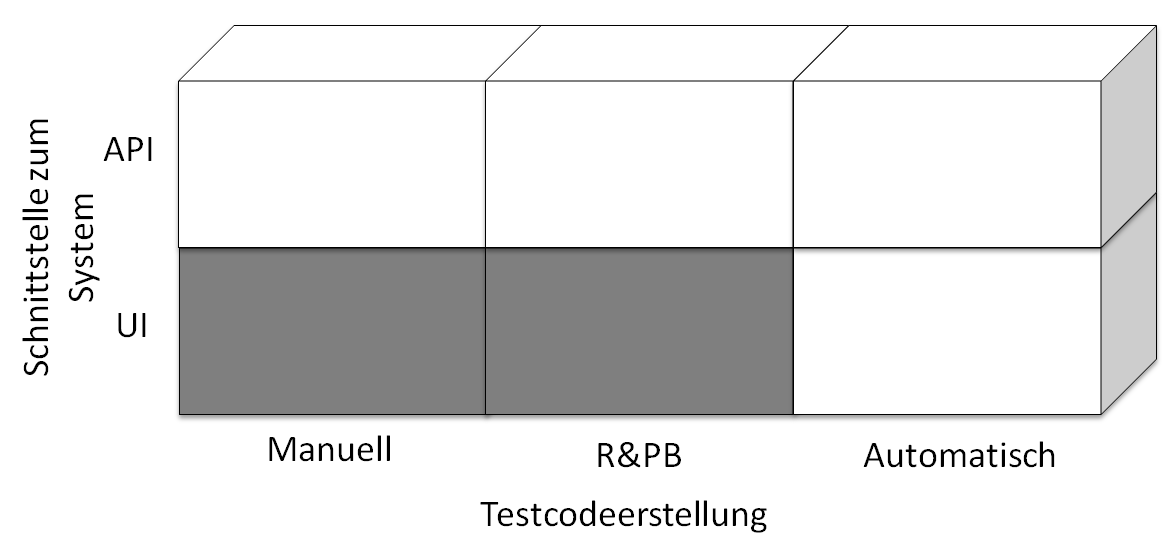
\includegraphics[scale=0.7]{img/bereicheTestcodeerstellungSelenium.png}\\
  \footnotesize\sffamily\textbf{Quelle:} vgl. \cite{meszaros_agile_2003}
  \caption{Einordnung von Selenium in die verschiedene Möglichkeiten der Testcodeerstellung}
  \label{fig:bereicheTestcodeerstellungSelenium}
\end{figure}
Genau genommen handelt es sich bei Selenium aber nicht um ein einzelnes Tool, sondern um eine Reihe von Tools die unter dem Namen Selenium zusammengefasst werden.
In seiner aktuellen Ausprägung 2.x lassen sich, abgesehen von Komponenten die der Abwärtskompatibilität dienen, laut Dokumentation \cite{selenium_selenium_2015-1} drei Komponenten unterscheiden:

\begin{itemize}
\item Selenium IDE \\
Bei der Selenium IDE handelt es sich um ein Firefox plug-in, das verwendet werden kann um Selenium-Testscripte zu erstellen. Testscripte können dabei von Hand erstellt oder mittels eines \grq record-and playback\grq -Mechanismus direkt im Browser aufgezeichnet werden. Die erstellten Testfälle können mit Akzeptanzkriterien angereichert werden und innerhalb der IDE wieder abgespielt werden.
\item Selenium WebDriver \\
Der Selenium WebDriver bietet für verschiedene Programmiersprachen eine API zur Steuerung eines Browsers aus dem Programmcode heraus. Der WebDriver bildet damit die Kernkomponente für alle Selenium-Testfälle die außerhalb der Selenium IDE entwickelt werden.

\item Selenium Server/Grid \\
Mit Hilfe des Selenium Servers ist es möglich Selenium-Testfälle nicht nur auf dem eigenen Rechner auszuführen sondern die Ausführung auf einen Server auszulagern. Einen wichtigen Teil des Selenium Server bildet Selenium Grid. Selenium Grid bietet die Möglichkeit die Ausführung von Selenium-Testfällen über einen Server hinaus auf eine Vielzahl von Knoten zu verteilen. Selenium Server dient dann als Hub der die Testfallanfragen auf Registriert Knoten zur Ausführung weiterleitet. 
\end{itemize}


\section{Testdurchführung mit Selenium}
\label{sec:testdurchführung_mit_selenium}
Abhängig davon ob die Testfälle für die Selenium IDE entwickelt wurden oder sich auf den Selenium WebDriver stützen unterscheiden sich die Möglichkeiten zur Ausführung der Testskripte.\\
Testfälle die mit der Selenium IDE entwickelt wurden verwenden eine Selenium eigene Sprache mit dem Namen \grq Selense\grq.\ Diese Testfälle können in späteren Testläufen wieder über die Selenium IDE zur Ausführung gebracht werden. \\
Dem gegenüber stehen Testfälle die den Selenium WebDriver verwenden.
Testfälle die mittels Selenium WebDriver entwickelt wurden sind für ihre Ausführung nicht an ein spezielles Tool gebunden. Beim WebDriver handelt es sich um eine API mit deren Hilfe ein Browser ferngesteuert werden kann. Wie diese API in die Testfälle integriert wird ist dem Entwickler selbst überlassen. In der Praxis hat sich als Best Practice jedoch herausgestellt, dass Selenium-Testfälle, die den WebDriver verwenden, meist in Verbindung mit einem Unit Testing Framework entwickelt werden.
Im Java Umfeld wären hier beispielsweise JUnit oder TestNG zu nennen.
Die Testfälle können damit analog zu den klassischen Unit Tests entwickelt werden, verwenden jedoch als Schnittstelle zum System nicht die API sondern, über den WebDriver, die Benutzeroberfläche. 
Die Ausführung der Testfälle erfolgt dann analog zu den klassischen Unit Tests über das Unit Testing Framework.
Im Bereich des WebDrivers stützt sich Selenium also auf bereits sehr gut etablierte Frameworks. Das hat den Vorteil, dass die so erstellten Testfälle bereits in den meisten Programmiersprachen gut in die Infrastruktur integriert sind. In Java sind Testfälle die mittels JUnit ausgeführt werden in allen gängigen IDEs durch Plugins unterstützt. Noch viel wichtiger ist jedoch eine gute Integration der Testfälle in den Buildprozess. Werden beispielsweise in Java Standarttools wie Gradle oder Maven zum bauen der Projekte verwendet, können die Testfälle ohne Mehraufwand im Rahmen des Buildprozesses ausgeführt werden.



\section{Testcodeerstellung mit Selenium}
\label{sec:Testdesign}
Die Testcodeerstellung von Testfällen die Selenium verwenden kann auf zwei Arten erfolgen.
Testcode kann Manuell erstellt werden oder über einen \grq record-and playback\grq -Mechanismus teilautomatisiert generiert werden.

\subsection{Recorde-and-playback}
\label{sec:recorde_and_playback}
Die Selenium IDE bietet die Möglichkeit Testskripte mittels \grq record and playback\grq\ zu erzeugen.
Die im Testfall gewünschten Abläufe können dabei einfach im Browser abgearbeitet werden.
Die durchgeführten Schritte werden von der Selenium IDE in der Selenium eigenen Sprache \grq Selense\grq\ aufgezeichnet. Diese Aufzeichnungen können später von der Selenium IDE interpretiert werden um so die Testabläufe erneut zu wiederholt.
Testskripte können nach dem Aufzeichnen nachträglich überarbeitet werden. Damit können beispielsweise Akzeptanzkriterien an bestimmten Stellen im Testablauf eingearbeitet werden.\\
Testfälle die über den \grq record-and playback\grq -Mechanismus erstellt wurden sind nicht an die Sprache \grq Selense\grq\ gebunden. Die Selenium IDE bietet die Möglichkeit die Testskripte in eine Reihe von Programmiersprachen zu exportieren. Darunter beispielsweise auch Java.
Diese Testfälle benutzen dann wie in Abschnitt \ref{sec:testdurchführung_mit_selenium} beschrieben, den Selenium Webdriver für die Kommunikation mit dem Browser und ein Unit Testing Framework für die Ausführung.\\
Die \grq record and playback\grq -Funktionalität bietet eine besonders einfache und schnelle Möglichkeit um Testfälle zu erstellen. Dennoch wird in der Dokumentation von Selenium \cite{selenium_selenium_2015-1} davon abgeraten sich bei der Testfallerstellung alleine auf dieses Tool zu stützen. Die Selenium IDE wird als Prototyping-Tool verstanden mit dem kleine Aufgaben, die nicht für den längerfristigen Einsatz gedacht sind, schnell automatisiert werden können.
Testabläufe die über den \grq record-and playback\grq -Mechanismus in der IDE erstellt werden unterliegen eine Reihe von Limitierungen. Leotta et al. \cite{leotta_repairing_2013} nennen als Limitierungen dieser Testfälle das fehlen von bedingten Anweisungen, Schleifen, Logging, Ausnahmebehandlungen so wie parametrisierten (a.k.a. data-driven) Testfällen.
Neben diesen Limitierungen haben die Testfälle zusätzlich das Problem, dass sie eine schlechte Wartbarkeit aufweisen. Nach Leotta et al. \cite{leotta_repairing_2013} liegt das vor allem daran, dass die Testfälle sehr stark mit der Struktur der Webseiten verwoben sind und einen hohen Anteil an dupliziertem Code aufweisen.
Die Limitierungen der IDE können zwar durch das Exportieren der Testfälle in eine Programmiersprache überwunden werden, die Qualität der Testfälle im Bezug auf ihre spätere Wartbarkeit kann nach  Leotta et al. \cite{leotta_repairing_2013} auf diesem Wege jedoch nicht verbessert werden.\\
Um die starke Verwobenheit mit der Webanwendung und den hohen Anteil an dupliziertem Code zu veranschaulichen wurden zwei Testfälle über den \grq record-and playback\grq -Mechanismus von Selenium erstellt und in die Programmiersprache Java exportiert.
Die Beiden Testfälle sollen das anlegen und editieren eines Datensatzes auf einer einfachen Web-Anwendung überprüfen.
Drei Seiten der Webanwendung werden für diesen Testfall verwendet. Die Seiten sind in Abbildung \ref{fig:toDoApp} dargestellt.

\begin{figure}[htb]

 \subfigure[Anlegen eines neuen Datensatzes]{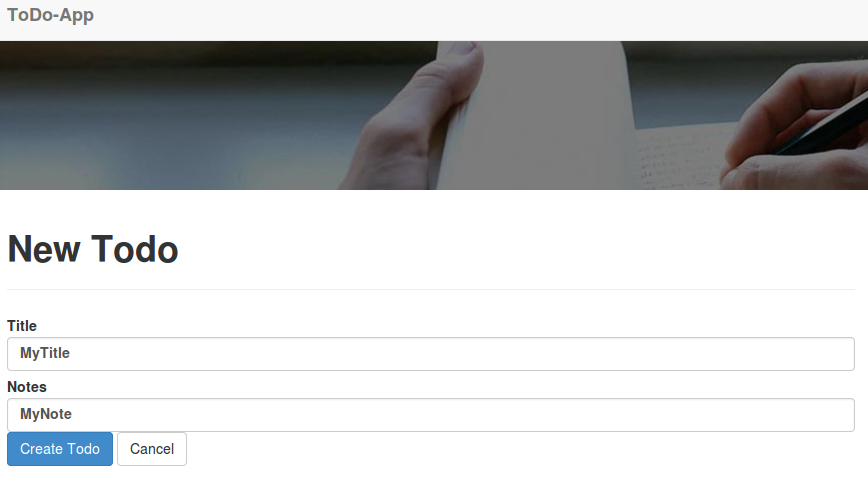
\includegraphics[width=0.49\textwidth]{img/newTodo.png}}
  \subfigure[Anzeigen eines Datensatzes]{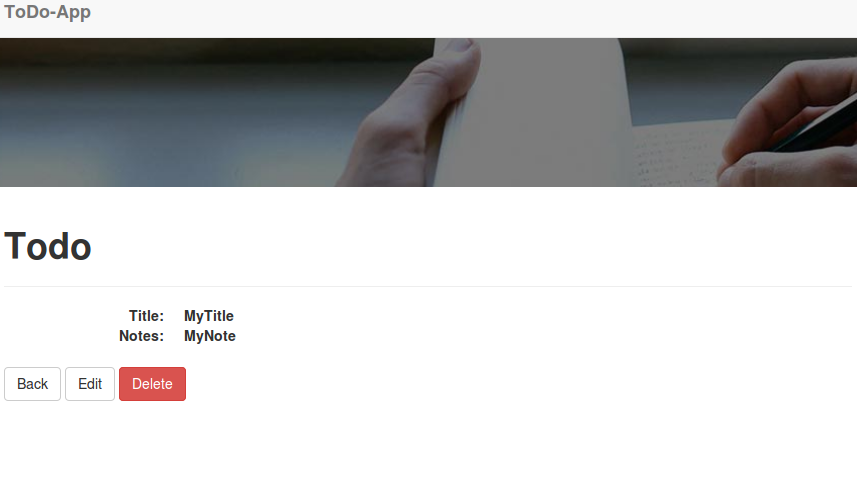
\includegraphics[width=0.49\textwidth]{img/showTodo.png}}
 \subfigure[Editieren eines Datensatzes]{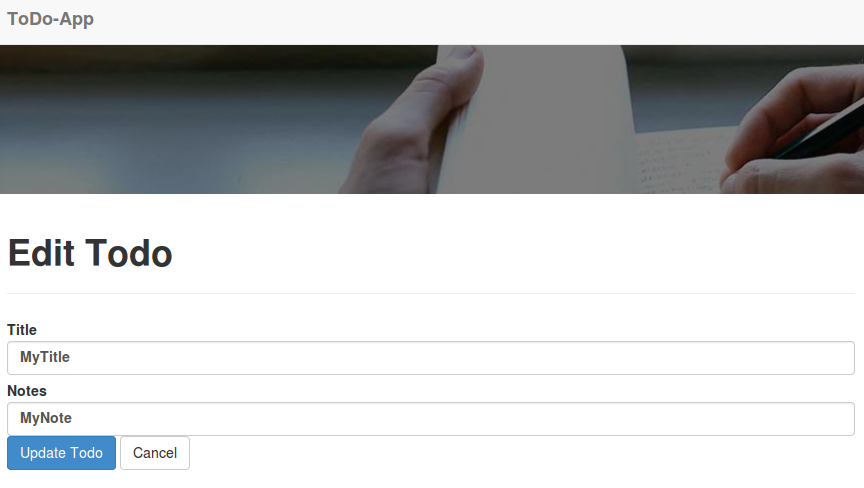
\includegraphics[width=0.49\textwidth]{img/editTodo.png}}
 \caption{Anlegen, Editieren und Anzeigen eines neuen Datensatzes}
  \label{fig:toDoApp}
\end{figure}


Zur besseren Lesbarkeit wurden die Testfälle im Listing \ref{lst:exportierteTestfaelle} leicht überarbeitet, in ihrem Wesen jedoch nicht verändert.
\begin{lstlisting}[caption={Exportierte Testfälle},label={lst:exportierteTestfaelle}]
  /**
  * Testfall legt einen neuen Datensatz an.
  */
  @Test
  public void testCreateNewRecord() {
    WebDriver driver = new FirefoxDriver();
    driver.get("http://localhost:3000/todos/new");
    driver.findElement(By.id("todo_title")).sendKeys("MyTitle");
    driver.findElement(By.id("todo_notes")).sendKeys("MyNote");
    driver.findElement(By.name("commit")).click();
  
    assertEquals("MyTitle", driver.findElement(By.id("title")).getText());
    assertEquals("MyNote", driver.findElement(By.id("note")).getText());
  }
  
  /**
  * Testfall legt einen neuen Datensatz an und editiert ihn.
  */
  @Test
  public void testEditRecord() {
    WebDriver driver = new FirefoxDriver();
    driver.get("http://localhost:3000/todos/new");
    driver.findElement(By.id("todo_title")).sendKeys("MyTitle");
    driver.findElement(By.id("todo_notes")).sendKeys("MyNote");
    driver.findElement(By.name("commit")).click();
    driver.findElement(By.linkText("Edit")).click();
    driver.findElement(By.id("todo_title")).clear();
    driver.findElement(By.id("todo_title")).sendKeys("MyTitleEdit");
    driver.findElement(By.id("todo_notes")).clear();
    driver.findElement(By.id("todo_notes")).sendKeys("MyNoteEdit");
    driver.findElement(By.name("commit")).click();
    
    assertEquals("MyTitleEdit", driver.findElement(By.id("title")).getText());
    assertEquals("MyNoteEdit", driver.findElement(By.id("note")).getText());
  }
  
\end{lstlisting}
Die Testfälle für das Anlegen und Editieren sind in ihren Abläufen recht ähnlich. Beide Testfälle legen zunächst einen neuen Datensatz in der Anwendung an. Die Logik die hierfür verwendet wird ist in beiden Testfällen dupliziert worden. Das ist nicht nur ein Problem dieses Beispiels sondern ein Problem, dass durchaus hohe Praxisrelevanz hat. In den meisten Testabläufen finden sich wiederkehrende Aufgaben, wie beispielsweise einen Login, der nicht nur von einem Testfall benötigt wird.
Selbst wenn sich die Abläufe zwischen den Testfällen stark unterscheiden werden Elemente, z.B. Input-Felder, die von der Anwendung angeboten werden in der Regel nicht nur einmal benutzt. Das führt zwangsläufig dazu, dass die Logik zum adressieren dieser Felder in einer Vielzahl von Testfällen dupliziert wird.\\
Die Adressierung der Elemente in der Anwendung bedingt auch die hohe Koppelung der im Listing \ref{lst:exportierteTestfaelle} gezeigten Testfälle mit den Seiten der Anwendung die Leotta et al. \cite{leotta_repairing_2013} als weiters problem identifiziert haben. Die Selektoren die verwendet werden um die Elemente der Webanwendung anzusteuern sind direkt in den Testfall eingearbeitet. Änderungen an der Seitenstruktur der Anwendung haben damit direkten Einfluss auf die Testfälle.\\
Obwohl sich die eigentliche Testfallspezifikation durch eine Änderung in der Seitenstruktur nicht ändert, müssen die Testfälle trotzdem überarbeitet werden.
Der duplizierter Code und der hohe Grad an Koppelung mit der Anwendung innerhalb der Testfälle bedingen, dass selbst kleine Änderungen in der zu testenden Anwendung, Korrekturen an vielen Stellen in den Testfällen nötig machen.

\subsection{Manuell}
\label{sec:manuell}
Eine weitere Möglichkeit bildet das manuelle Erstellen der Testskripte. Für die Ausführung und die Kommunikation mit der Anwendung verwenden die manuell erstellten Skripte das selbe Toolset wie die generierten und exportierten Testfälle aus der \grq record-and playback\grq -Variante. Analog zu den in Listing \ref{lst:exportierteTestfaelle} gezeigten Testfällen wird der Selenium WebDriver für die Kommunikation mit der Anwendung verwendet. Die Ausführung geschieht über ein Unit Testing Fraemwork.
Im Vergleich zu den halbautomatisch generierten Testfällen ist das manuelle entwickeln der Testskripte aufwändiger.
Es bietet jedoch die Möglichkeit die in Abschnitt \ref{sec:recorde_and_playback} genannten Problemen der \grq record-and playback\grq -Variante entgegenzuwirken.
Bei einem manuellen Ansatz kann von Anfang an auf eine wartbare und wiederverwertbare Struktur in den Testfällen geachtet werden.
Als best practice hat sich zu diesem Zwecke das Page Object Design Pattern durchgesetzt.

\subsection{Page Object Pattern}
\label{sec:page_object_pattern}
Im Page Object Pattern wird versucht die Funktionalität welche die zu testende Anwendung anbietet in einem objektorientierten Ansatz zu kapseln.
Alle Seiten der zu testenden Anwendung werden dazu als Objekte Modelliert. Auf diese Weise wird die Funktionalität die von einer Seite angeboten wird zu einem Service, beispielsweise einer Methode, die von dem korrespondierendem Page Object angeboten werden.
Alle Informationen und Funktionalität die von einer Seite angeboten werden sind so zentral gekapselt.
Ein Page Objekt ist also eine objektorientierte Klasse die als Interface für eine Seite der zu testenden Anwendung dient.
Sämtliche Interaktion mit der zu testenden Anwendung geschieht über die in den Page Objekten angeboten Schnittstellen.
Änderungen an der Oberfläche der zu testenden Anwendung haben so keinen direkten Einfluss mehr auf die Testfälle. Bei Änderungen an der Benutzeroberfläche muss nur noch Code an einer Stelle innerhalb der Page Objekte angepasst werden.\\
Um das Zusammenspiel zwischen Page Objekten und Testfall besser zu verdeutlichen wurde der Testfall zum anlegen eines neuen Eintrags aus Listing \ref{lst:exportierteTestfaelle} im Page Object Pattern nachgebaut.

Der Testfall Arbeitet mit zwei Seiten der Anwendung. Die Seiten sind in Abbildung \ref{fig:toDoApp} dargestellt. Für jede der beiden Seiten wird ein Page Object als Kommunikationsschnittstelle benötigt. 
Das Page Object CreatPage in Listing \ref{lst:poCreatePage} repräsentiert die Seite zum anlegen eines neuen Datensatzes (Abbildung \ref{fig:toDoApp} a). Das Page Object ShowPage in Listing \ref{lst:poShowPage} repräsentiert die Seite zum anzeigen eines Datensatzes (Abbildung \ref{fig:toDoApp} b).

\begin{lstlisting}[caption={Page Object CreatePage},label={lst:poCreatePage}]
  public class CreatePage extends BasePo {
		public final Control tfTodotitle = control(by.textField("todo_title"));
		public final Control tfTodonotes = control(by.textField("todo_notes"));
		public final Control bCreateTodo = control(by.button("commit"));

		public CreatePag(PageObject po) {
			super(po);
		}
		public ShowPage createEntry(String title, String note){
			tfTodotitle.sendKeys(title);
			tfTodonotes.sendKeys(note);
			bCreateTodo.click();
			return new ShowPage(this);
		}
  }
\end{lstlisting}  
\begin{lstlisting}[caption={Page Object ShowPage},label={lst:poShowPage}]  
  public class ShowPage extends BasePo {
		public final Control idTitle = control(by.id("title"));
		public final Control idNotes = control(by.id("note"));

		public ShowPage(PageObject po) {
			super(po);
		}
  }
\end{lstlisting}

Die Funktionalitäten die von den jeweiligen Seiten angeboten werden sind innerhalb des Page Objects gekapselt. Das Page Object CreatPage bietet beispielsweise die Eingabefelder für Titel und Note so wie den Button zum anlegen eines Datensatzes als globale Objekte von Typ Control an.
Die Klasse Control dient in den dargestellten Page Objekten als Wrapper für den Selenium WebDriver. Control-Objekte sind also analog zu Selenium WebElementen zu verstehen.
Die Funktionalität zum anlegen eines neuen Eintrags die im späteren Testfall benötigt wird bietet das Page Objekt CreatPage als Service-Methode \grq createEnty()\grq\ an.\\

Der Testfall in Listing \ref{lst:pageObjectTestfall} verwendet die Beiden Page Objekte um einen neuen Eintrag in der Anwendung anzulegen und zu überprüfen.


\begin{lstlisting}[caption={Page Object Testfall},label={lst:pageObjectTestfall}]  
  /**
  * Testfall legt einen neuen Datensatz an.
  */
 	@Test
	public void testCreateNewRecord(){
		CreatePage createPage = new CreatePage(po);
		ShowPage showPage = createPage.createEntry("MyTitle", "MyNote");

		assertEquals("MyTitle", showPage.idTitle.resolve().getText());
		assertEquals("MyNote", showPage.idNotes.resolve().getText());
	}

\end{lstlisting}

Im Gegensatz zum Testfall in Listing \ref{lst:exportierteTestfaelle} ist es auf Grund des Page Object Pattern nicht mehr nötig explizite Referenzen auf die Struktur der Seite innerhalb der Testfälle zu machen. Alle Details der Seite sind innerhalb der PageObjekte gekapselt. Der Testfall verwendet lediglich die im Page Object angebotenen Funktionalität.


\subsubsection{Vorteile des Page Object Pattern}
\label{sec:vorteile_des_page_object_pattern}

Folgende Vorteile ergeben sich damit bei der Verwendung des Page Object Pattern die auch so in der Selenium Dokumentation \cite{selenium_selenium_2015-2} angegeben werden:

\begin{enumerate}
\item Es gibt eine klare Trennung zwischen Testcode und seitenspezifischem Code wie beispielsweise Elementadressierungen und Layout. \\ \\
Die Adressierung der Elemente ist nicht mehr über die gesamten Testfälle verteilt sondern befindet sich an einem zentralen Ort, dem Page Object.
Die hohe Koppelung der Testfälle mit den Seiten der Anwendung die Leotta et al. \cite{leotta_repairing_2013} als Problem genannt haben kann somit überwunden werden.

\item Es gibt einen einzigen Ort für die Elemente und Operationen die von einer Seite angeboten werden. \\ \\
Alle Informationen die eine Seite der Anwendung betreffen sind an einem zentralem Ort, dem Page Object gesammelt. Seitenspezifischer Code muss somit nicht mehr in den einzelnen Testfällen dupliziert werden. Die Funktionalitäten der Seite können über das entsprechende Page Object abgerufen werden.

\end{enumerate}

Beide Vorteile führen dazu, dass Änderungen die an einer Seite gemacht werden nur Auswirkungen an einem zentralen Stelle haben. Die Wartbarkeit der gesamten Testfälle wird so erhöht.
Leotta et al. unterstützen diese These mit einer Fallstudie \cite{leotta_repairing_2013} in der Sie eine herkömmliche Testsuite mit einer Testsuite die das Page Object Pattern implementiert hinsichtlich ihrer Wartbarkeit verglichen haben.
Das Ergebnis dieser Studie hat gezeigt, dass in Ihrem Fall die Zeit für die Wartung der Testfälle um ca. 65\% reduziert werden konnten. Die Anzahl der anzupassenden Codezeilen konnte um ca. 87\% reduziert werden.

\subsubsection{Probleme des Page Object Pattern}
\label{sec:probleme_des_page_object_pattern}

Die Vorteile des Page Object Pattern kommen allerdings mit einem Preis. Die Komplexität des gesamten Testprojekts steigt. Testfälle können nicht mehr beliebig programmiert werden sondern sind in den Kontext von Page Objekts zu stellen. Das erfordert tiefgründige Designentscheidungen. So ist beispielsweise zu klären wie über die Page Objekts ein generischer Einstieg in die Anwendung angeboten werden kann oder wie der WebDriver über mehrere Page Objekts und Testfälle hinweg verwaltet werden kann. Auch die Page Objects selbst müssen erst einmal entwickelt werden bevor mit dem erstellen von Testfällen begonnen werden kann.\\
Verglichen mit einem herkömmlichen Ansatz steigt mit der Verwendung des Page Object Pattern zu Beginn also der Aufwand beim erstellen eines Testprojektes. Leotta et al. \cite{leotta_repairing_2013} haben gezeigt, dass sich diese Investition durchaus lohnen kann, initial sind die Kosten allerdings höher.
